\documentclass[12pt]{article}

\usepackage{graphicx}
\graphicspath{{figures/}} % Location of the graphics files
\usepackage[font=small,labelfont=bf]{caption} % Required for specifying captions to tables and figures
\usepackage{amsfonts, amsmath, amsthm, amssymb}
%\usepackage{wrapfig}
\usepackage{indentfirst}

\begin{document}
\title{HAPIEST User Manual} 
\date{}
\maketitle
\thispagestyle{empty}
\newpage

\tableofcontents
\thispagestyle{empty}
\newpage

\setcounter{page}{1}
\section{HAPIEST}
HITRAN Application Programming Interface and Efficient Spectroscopic Tools (HAPIEST) is a GUI for the HITRAN Application Programming Interface (HAPI). HAPIEST's development began at SUNY Oswego in a software engineering course by students Benji Caro, Joshua Karns, Dominik Lohmann, Wyatt Matt, Ethan Messer, and Michael Sova, and in conjunction with Dr. Iouli Gordon and Dr. Roman Kochanov of the Harvard-Smithsonian Center for Astrophysics and under advisement of SUNY Oswego professor Bastian Tenbergen and SUNY Oswego Professors and Head of Physics Department Shashi Kanbur. HAPIEST functions as a GUI for HAPI.
\subsection{Program Overview}
The goal of HAPIEST is to simplify the use of the HITRAN Application Programming Interface (HAPI) for all users. Currently, HAPI requires some knowledge of Python and use of the command line. HAPIEST should retain as much of the funtionality HAPI as is possible in a simple GUI, while making it easier to access and use for the user. HAPIEST currently allows users the capability to fetch/download and locally store data from the HITRAN database, edit local data, and also to generate and plot spectral functions. In it's current form, HAPIEST is split up into 3 windows, one window for data management and editing, and two windows for graphing/graph display.

\section{Main Window}
The Main Window provides the functionality of HAPI and is split into several tabs each focusing on a different feature/function. 
\subsection{Fetch Tab}
The Fetch tab allows the user to download data from HITRAN onto their local disk for the available molecules and their supported isotopologues. Further, the user can select from the Parameter Groups list and Parameters list to download more specific data. This window is the users primary method of obtaining data.
\begin{center}
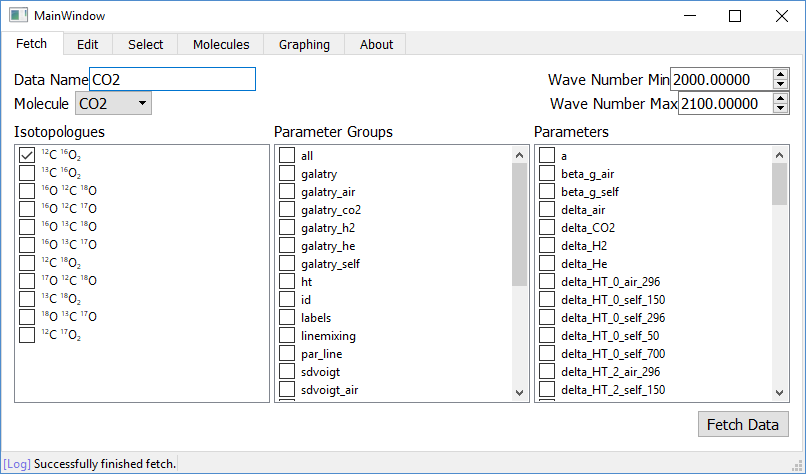
\includegraphics[scale = 0.6]{MainWindow_Fetch}
\end{center}
\subsubsection{Fetch Dictionary}
\begin{itemize}
\item Data Name - Local file name of data being downloaded.
\item Molecule - List of molecules to select which Isotopologues to fetch data for, updates the Isotopologues list when a molecule is selected.
\item Wave Numer Min - Lower threshold to fetch data (from).
\item Wave Number Max - Upper threshold to fetch data (to).
\item Isotopologues - List of Isotopologues for the selected molecule. This is what you are fetching data for.
\item Parameter Groups - List containing groups of spectral line parameters.
\item Parameters - List of individual spectral line parameters to fetch for selected isotopologues.
\end{itemize}

\subsection{Edit Tab}
The edit tab allows users to view and edit local data that has been downloaded through HAPIEST. It offers a table view of all parameters and values, and can be saved to disk.
\begin{center}
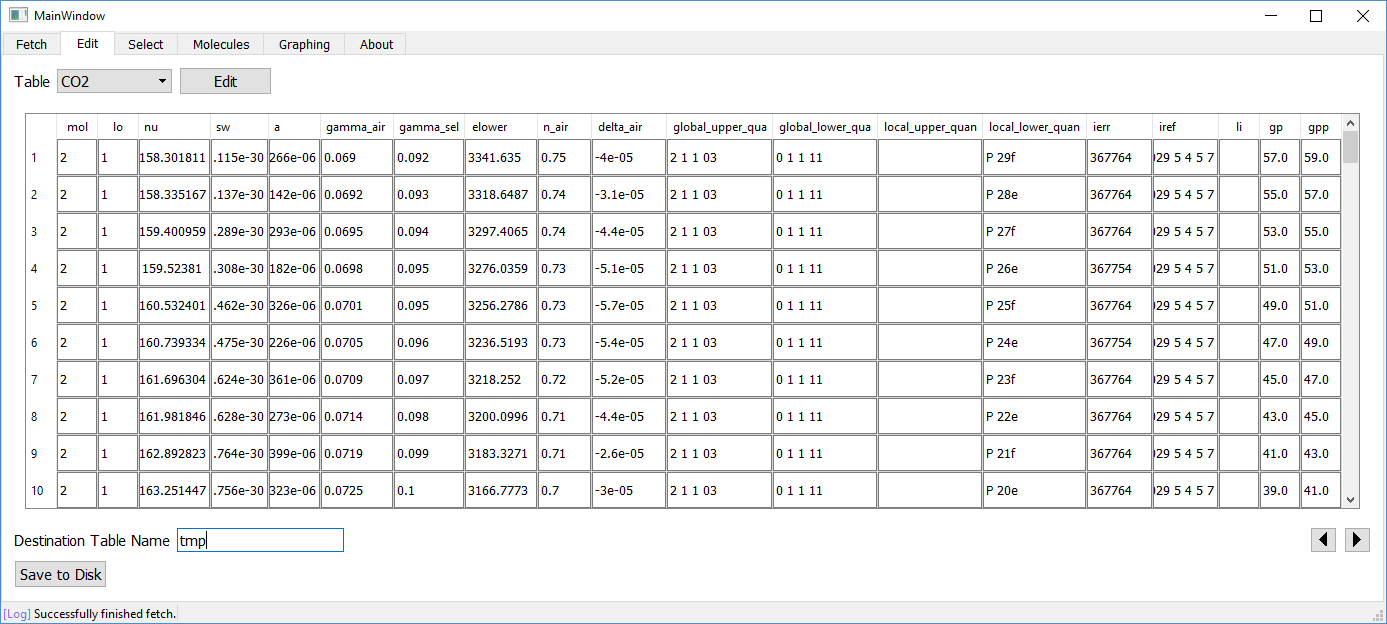
\includegraphics[scale = 0.4]{MainWindow_Edit}
\end{center}
\subsubsection{Edit Dictionary}
\begin{itemize}
\item Table - List of HITRAN data files.
\item Edit - Button that populates table containing information in the data file.
\item Destination Table Name - Name of local file upon saving.
\item (Left and Right Arrows) - Select between pages of data.
\item Save to Disk - Button that saves the  current table to disk.
\end{itemize}

\subsection{Select Tab}
The select tab is dedicated to the fetch method call available in HAPI and allows users a more advanced fetch.
\begin{center}
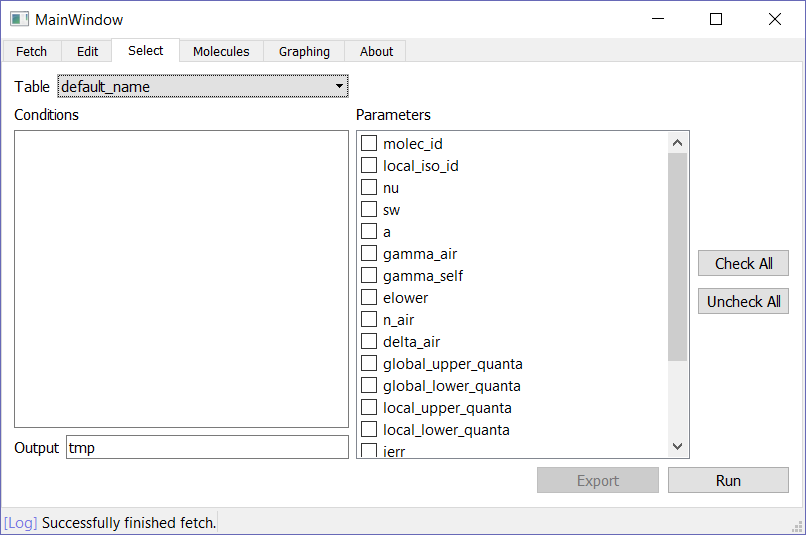
\includegraphics[scale = 0.6]{MainWindow_Select}
\end{center}

\subsection{Molecules Tab}
The molecules tab provides reference for the available molecules and also reference ids for each molecule.
\begin{center}
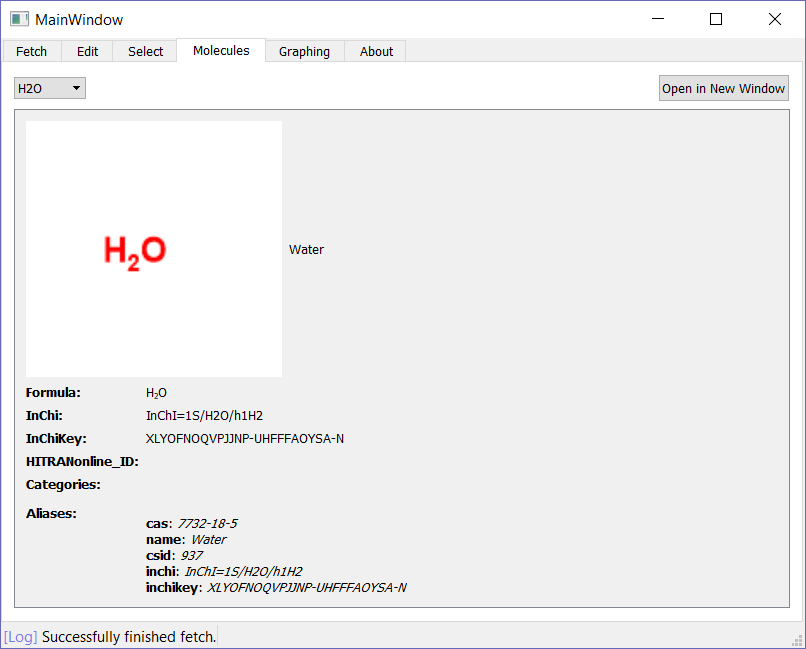
\includegraphics[scale = 0.6]{MainWindow_Molecules}
\end{center}

\subsection{Graphing Tab}
In the graphing tab, the user is given a list of parameter fields to populate in order to create the specific graph they need for each graph type (Absorption Coefficient; Absorption, Transmittance, and Radiance Spectra graphs). Multiple plots of the same type may be displayed together on the same graph.
\begin{center}
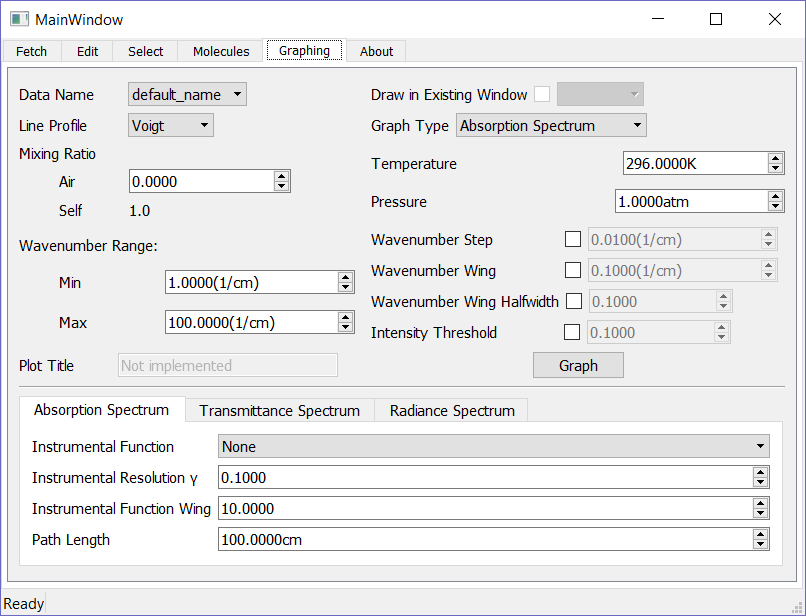
\includegraphics[scale = 0.6]{MainWindow_Graphing}
\end{center}
\subsubsection{Graphing Dictionary}
\begin{itemize}
\item Data Name - Data file used to calculate spectra for graphing.
\item Draw in Existing Window - Checkbox to enable multiple plots on the same graph for the same Line Profiles. List of graph windows open to plot to.
\item Line Profile - Line profile (lineshape) type to use in the spectra calculation..
\item Graph Type - Type of the graph to plot: dependent on the spectra type (i.e. absorption, transmittance, etc...).
\item Mixing Ratio - Volume mixing ratio of air in the modeled mixture.
\item Temperature - Temperature (Kelvin) of the modeled gas mixture.
\item Pressure - Total pressure (in atmospheres) of the modeled gas mixture.
\item Wave Number Range - Spectral range to be used in the simulation (in wavenumbers)
\item Wave Number Step - Wavenumber step to be used in the simulation.
\item Wave Number Wing - Absolute size of the wing (in wavenumbers) at which line profile is not zero.
\item Wave Number Wing Halfwidth - Relative of the size of the wing (in line halfwidths) at which line profile is not zero.
\item Intensity Threshold - Minimum value of the line intensity to consider in the spectra calculation.
\item Plot Title - Title of the plot.
\item Graph - Button that creates a plot according to selected parameters.
\end{itemize}

\subsection{About Tab}
The about tab is a summary tab informing the user about the development and some information about each tab.

\section{Graph Window}
Graphs are displayed in this window. There is an option in the graphing tab to display multiple graphs in the same window.
\subsection{User Interactivity}
File - Contains saving options.
View - Resets the view.
X and Y -
\subsubsection{Box Zoom}
To box zoom, simply click the left mouse button, hold it down and drag across the area you want to zoom in on, and release. In order to reset the graph view, click View in the menu and then click Fit.
\begin{center}
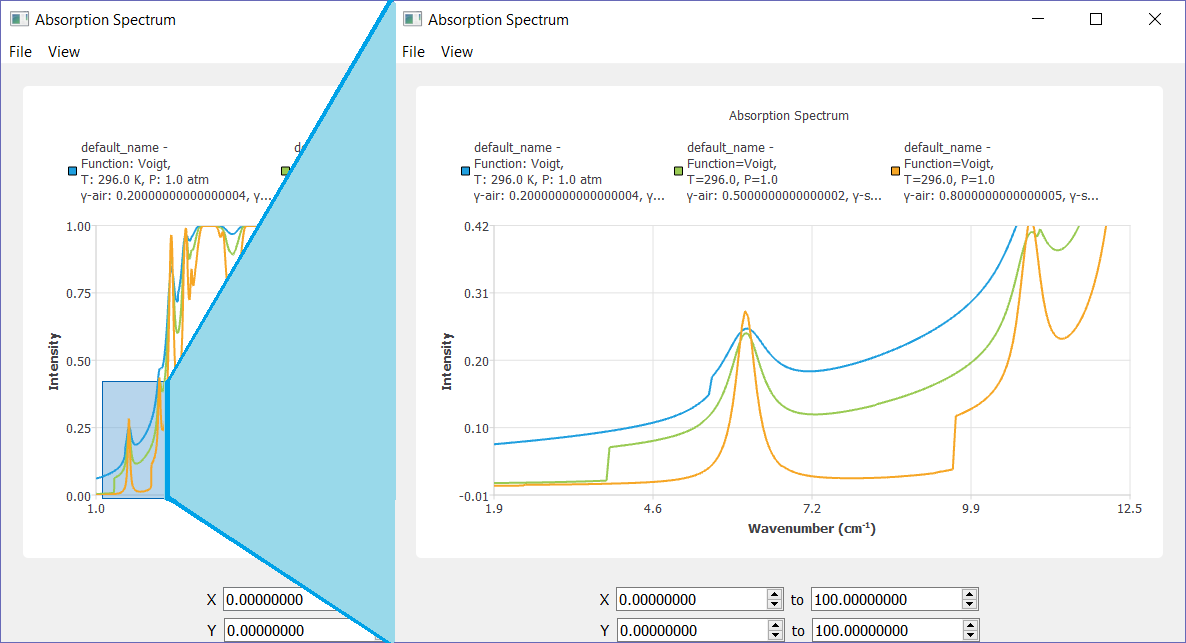
\includegraphics[scale = 0.5]{GraphDemo}
\end{center}
\subsubsection{Save Features}
Options to save graphs in image formats PNG and JPEG, or  text based as Comma Separated Values (CSV), Text File (TXT), or in JSON format.
%\includegraphics{}

\section{How to Use}
\subsection{Fetching Data}
In order to plot/graph data, the user needs to first download data from the HITRAN database. This can be done in HAPIEST or using HAPI. To do so in HAPIEST, follow the instructions below.
\begin{center}
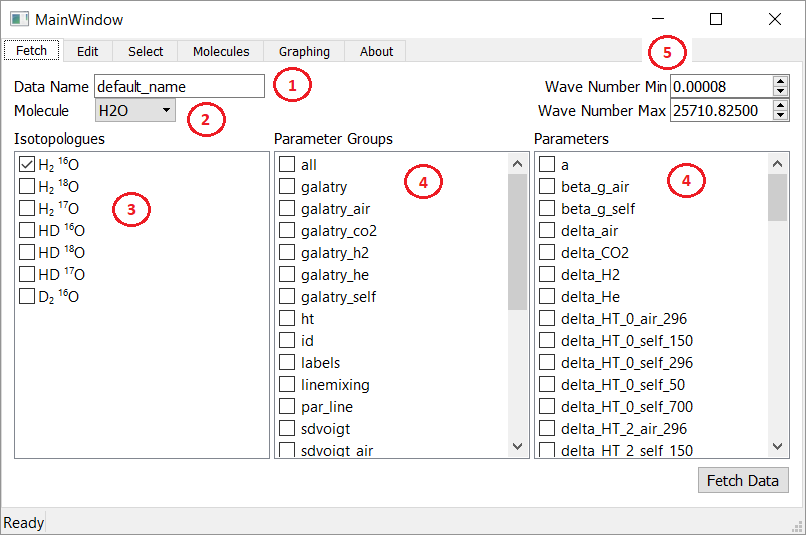
\includegraphics[scale = 0.5]{MainWindow_FetchGuide}
\end{center}
\begin{enumerate}
\item Edit data name to change the name of the file downloaded upon fetching.
\item Select the molecule to update the Isotopologues list.
\item Select the Isotopologues you want to download data for.
\item Select from the Parameter Groups and Parameters list to download further data for the selected Isotopologues.
\item Edit the Wave Number Min and Max values to refine your download (Smaller ranges are faster to fetch and take up less space).
\end{enumerate}

\subsection{Graphing Data}
Once you have data on your system, you can then go to the Graphing Tab to produce a graph. 
\begin{center}
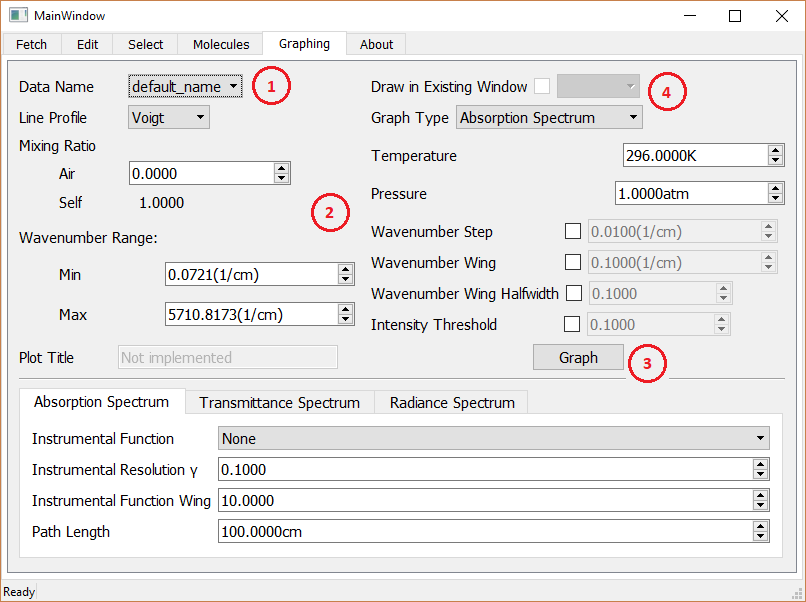
\includegraphics[scale = 0.5]{MainWindow_GraphingGuide}
\end{center}
\begin{enumerate}
\item In the Data Name list, select the data file you want to use to create a plot.
\item Skip Draw in Existing Window for now, and select the parameters of the plot.
\item Click the graph button and another window will appear to display the graph.
\item Now, if you want to plot another graph of the same type in/with a previous plot, check the Draw in Existing Window check box and select the compatible window in the drop-down list.
\end{enumerate}


\section{Demo}
\end{document}
